\subsection{Front and Rear Distance}
\label{subsec:03_distance}

% \change[]{Image! Coordinate is not correct for set coordinate system}

% For simplicity, the direction of the sound source is determined in
% horizontal plane only.
% However, the front and rear microphones differ 0.0212\si{m} in height
% what can provide rough 
For the particular case when the signal comes straight from the front or behind,
the distance of the sound source can be estimated\todo{estimated und approx. haben die selbe Aussage}.
If $delay_{01}$ (delay between channel 0 and 1) and $delay_{32}$ (delay between channel 3 and 2)
are both very small, the signal comes from
the front or the back most likely. \todo{why "most likely" i think you can skip that and say it comes from front or back} \todo{comes most likely from the fround or rear.}
In theory, for this case the lateral delays are larger or equal the maximal
sample difference between the front and rear channels on the x-axis which is
to\todo{to?} 5.41 samples.
With smaller lateral delays and some assumptions \todo{the assumptions given below / or which assumptions are you talking about?}, the angle of the sound source in the XZ
plane can be estimated.
\Cref{fig:02_headSideTdoa} illustrates the NAO's head from the right with
channels 1 and 3.
% -------------------------------------------------------------
\begin{figure}[ht]
	\centering
		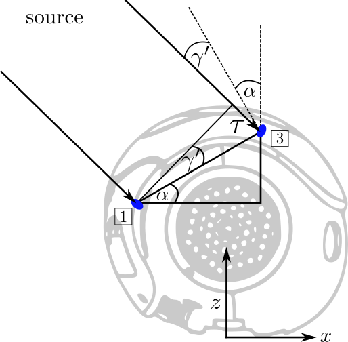
\includegraphics[width=0.45\columnwidth]{figures/side_head_tdoa}
    \caption{Illustration of arriving sound for sources from near behind.
             Adapted from \cite{nao_docu}.}
    \label{fig:02_headSideTdoa}
\end{figure}
% -------------------------------------------------------------

Assuming, that $delay_{01}$ and $delay_{32}$ are small,
the angle of the sound source $\gamma$ relative
to the Z-axis can be determined with delay $D$ as
% -------------------------------------------------------------
\bsub \bal
\gamma &= \alpha + \gamma'\\
\gamma' &= sign(D) \cdot sin^{-1}\left(\frac{D}{D_{max}}\right)\\
\intertext{whereby}
\alpha &= tan^{-1}\left(\frac{\Delta z_{channel}}{\Delta x_{channel}}\right) \approx 26.73\si{\degree}
\eal \esub
which is the angle to the orthogonal axis to \todo{zweimal to? muss da von einmal eins "from..." .."to.." sein? So ergibt sich mir die Aussage nicht } the plane though
front and rear channels.
$\Delta z_{channel}$ and $\Delta x_{channel}$ are the distances between the channels
in z- and x-direction in \si{\meter}.
% -------------------------------------------------------------
\begin{figure}[ht]
	\centering
		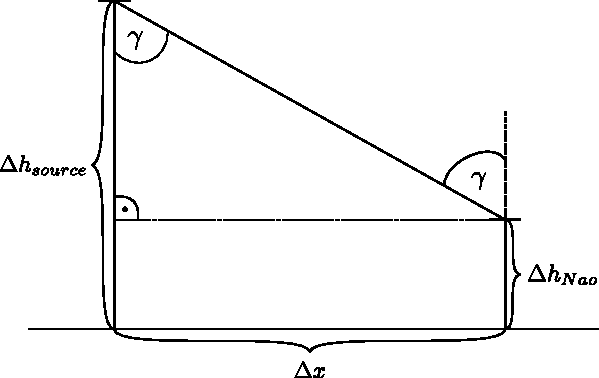
\includegraphics[width=0.6\columnwidth]{figures/x_distance}
	\caption{Illustration of distance estimation.}
    \label{fig:02_xDistance}
\end{figure}
% -------------------------------------------------------------

Knowing that the sound source is ordinarily positioned above of the robot, the distance
of the sound source can be approximated with an assumed height $\Delta h_{source}$
of the source. $\Delta h_{source}$ differs from referee and thus, can only be guessed.
So, the distance in x-direction $\Delta x$ is
% -------------------------------------------------------------
\bal
\Delta x &= (\Delta h_{source} - \Delta h_{NAO}) \cdot \tan(\gamma).
\label{eq:02_deltaX}
\eal
% -------------------------------------------------------------

The distance estimation is triggered, if the direction candidates of
$delay_{01}$ and $delay_{32}$ are smaller than $\pm$ 10\si{\degree}
or larger than $\pm$ 170\si{\degree}.
Additionally, the lateral delays must be smaller than 5.41 samples as mentioned above.

Restrictions of the front and rear distance measurement differ.
For the front case, the maximum angle for an unambiguous distance calculation
is $\frac{\pi}{2}- 2\alpha$.
Thus, the maximum front distance that can be approximated shrinks to
$\Delta x = (\Delta h_{source} - \Delta h_{NAO}) \cdot \tan(\frac{\pi}{2} - 2\alpha)$
according to \cref{eq:02_deltaX}.
To the rear, the maximal value for $\gamma$ is bounded by the 5.41 samples that
are set as condition.
Setting $\Delta h_{source}$ to 1.5\si{m} and $\Delta h_{NAO}$ to 0.57\si{\meter} for example,
the maximal measurable distance to the front is about 0.66\si{\meter}.
With the same values the maximal distance backwards is 15.3\si{\meter} in theory.
However, measurements in \cref{subsec:04_distance} show that 7\si{\meter} is the
limit for the real case. \todo{ich würde hier nochmal etwas klarer darstellen, woher der Unterschied zwischen front und rear kommt. Ist für dich vielleicht klar, für den Lesen, gerade beim ersten Mal aber nicht. Ein sollte da als Begründung reichen}

% -------------------------------------------------------------

\subsection{SNR}
\label{subsec:03_snr}

The \acf{SNR} is a common value to express the signal power $P_{signal}$ compared
to power of the background noise $P_{noise}$.
Conveniently, the buffered audio signal in this thesis always consists of
a clean-cut delimitation between signal and noise which is set by the
start index.
Thus, the \ac{SNR} which is defined as
\bal
    SNR_{db} = 10\log_{10}\left(\frac{P_{signal} - P_{noise}}{P_{noise}}\right)
    \label{eq:03_snr}
\eal
in decibels can be implemented straightforwardly.
Informational content about this measure is investigated in \cref{subsec:04_snr}.
Expectations are that the \ac{SNR} can be fed into the covariance matrix
of an incoming result in the Bayesian update process introduced in \cref{subsec:02_2dTeam}.

\subsection{PSNR}
\label{subsec:03_psnr}
In image processing, the \acf{PSNR} indicates the quality of a compressed
image. Here in this work, the ratio between the peak of a signal
and its noise is related to the \ac{GCC-PHAT} outcome and called \ac{PSNR}
henceforth.
As stated in \cref{sec:02_gcc}, the most significant characteristic
of the \ac{GCC-PHAT} is the resulting sharp peak which now can be
assessed with one value
\bal
    PSNR_{db} = 10\log_{10}\left(\frac{P_{peak}}{P_{noise}}\right).
    \label{eq:03_psnr}
\eal
From the implementation view, the power of the correlation peak is divided by
the power of the remaining correlation signal.
It has to be noted that two adjacent values prior and after the peak
are disregarded as they might belong to the peak.
A validation if and how much the \ac{PSNR} and the accuracy of the \ac{GCC}
delay result are linked is done in \cref{subsec:04_psnr}.